% Supplementary Material for:
% A Variance-Retention Diagnostic for Persistence-Relative Skill in Daily PM$_{10}$ Forecasting

\subsection*{S1. PRISMA reporting audit (supporting motivation)}
\begin{table}[htbp]
\centering
\caption{Abstract-level reporting visibility of evaluation-relevant practices in PM forecasting studies. Percentages are computed over 486 abstract-coded studies; low reporting rates indicate reporting opacity, not confirmed absence of the corresponding practice in full text.}
\label{tab:prisma-reporting-audit}
\begin{tabular}{llrl}
\toprule
Evaluation dimension & Explicitly reported & \% & Interpretive function \\
\midrule
Persistence or naive baseline & 18/486 & 3.7 & Minimum operational comparator \\
Horizon-wise reporting & 11/486 & 2.3 & Multi-step interpretability \\
Temporally appropriate validation & 24/486 & 4.9 & Deployment-like temporal credibility \\
Explicit leakage-safe safeguards & 3/486 & 0.6 & Protection against information bleed \\
Operational-usefulness framing & 51/486 & 10.5 & Decision relevance \\
\bottomrule
\end{tabular}
\end{table}


\begin{figure}[t]
\centering
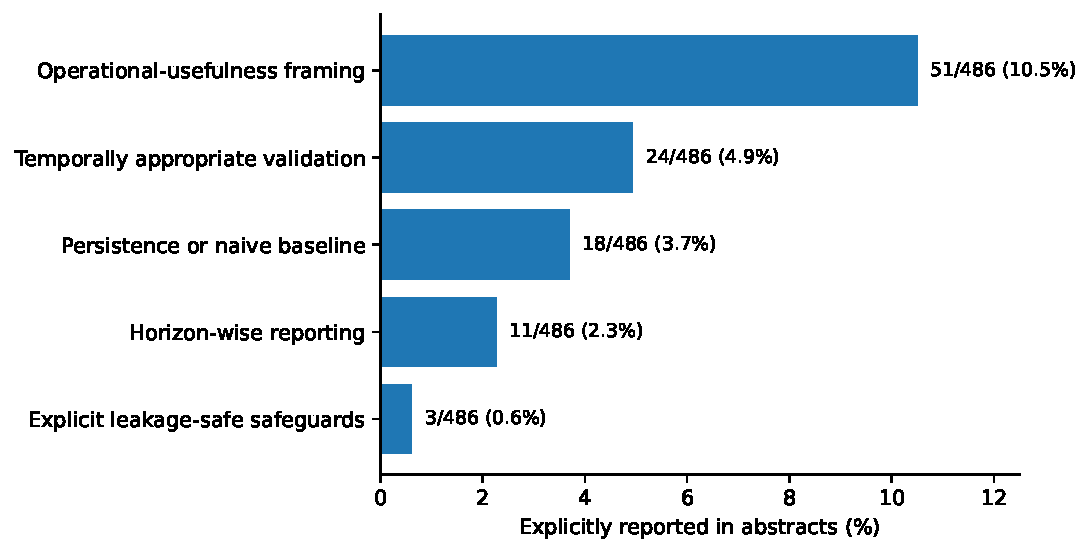
\includegraphics[width=0.92\linewidth]{figure1_reporting_gap_audit.pdf}
\caption{Abstract-level reporting visibility of key evaluation practices in particulate matter forecasting studies. Percentages are computed over 486 abstract-coded studies. Low percentages indicate reporting opacity, not confirmed absence of the corresponding practice in the full text.}
\label{fig:reporting-gap-audit-supp}
\end{figure}

\clearpage

\subsection*{S2. Monitoring stations}
\begin{table}[ht]
\centering
\small
\setlength{\tabcolsep}{3pt}
\caption{Monitoring stations included in the study. Stations span industrial,
  traffic, urban background, suburban, and rural remote settings within the
  MITECO national air-quality network. Coverage refers to available daily PM$_{10}$
  observations within the study period (2017--2024).}
\label{tab:stations-supp}
\begin{tabular}{@{}l>{\raggedright\arraybackslash}p{3.8cm}>{\raggedright\arraybackslash}p{3.3cm}rr@{}}
\hline
Station code & Name & Area type & Altitude (m a.s.l.) & Coverage (\%) \\
\hline
ES0446A & Elx-Agroalimentari & Suburban/Industrial & 44 & 80.4 \\
ES1619A & Valencia-Vivers & Urban/Residential & 11 & 91.7 \\
ES0012R & Zarra-EMEP & Rural Remote EMEP & 855 & 96.0 \\
ES1870A & Barcelona El Port Vell & Suburban/Industrial & 1 & 98.5 \\
ES1418A & Alagon & Suburban/Traffic & 235 & 97.5 \\
ES1421A & Teruel & Urban/Background & 915 & 96.7 \\
ES0001R & San Pablo de los Montes & Rural Remote/Background & 923 & 96.1 \\
ES1438A & Barcelona L'Eixample & Urban/Traffic & 26 & 95.3 \\
ES0567A & Barcelona Zona Universitaria & Urban/Background & 24 & 95.2 \\
ES1417A & Huesca & Urban/Traffic & 488 & 95.0 \\
ES0691A & Barcelona El Poblenou & Urban/Background & 3 & 94.9 \\
ES0559A & Barcelona Pl. Universitat & Urban/Traffic & 24 & 94.9 \\
ES1856A & Barcelona Vall d'Hebron & Urban/Background & 136 & 94.5 \\
ES1966A & Alcaniz Capuchinos & Urban/Industrial & 340 & 94.3 \\
ES2011A & Sant Vicenc dels Horts Alaba & Suburban/Industrial & 65 & 94.1 \\
ES2091A & Alcanar Montecarlo & Rural Remote/Industrial & 6 & 93.7 \\
ES2017A & Alcanar Llar de Jubilats & Rural Near-city/Industrial & 7 & 93.6 \\
\hline
\end{tabular}
\end{table}
